% The corpus's synthetic features paper: what arXiv papers rarely have (arXiv builds with pdfLaTeX) but Taudot users
% will: OpenType fonts through fontspec, transparency, rotated content, raw PDF specials, a Type 1 font beside them.
\documentclass[11pt]{article}
\usepackage[margin=1in]{geometry}
\usepackage{fontspec}
\usepackage{tikz,graphicx,xcolor}
\newfontfamily\cmr{lmroman10-regular.otf}
\newfontfamily\sans{texgyreheros-regular.otf}
\begin{document}
\section*{OpenType and Type 1}
{\cmr Latin Modern Roman (OpenType): The quick brown fox jumps over the lazy dog. fi fl ffi.}\par
{\sans TeX Gyre Heros (OpenType): Sphinx of black quartz, judge my vow.}\par
{\fontspec{texgyrepagella-regular.otf}[Numbers=OldStyle] Pagella with old-style figures 0123456789.}\par
$\displaystyle \int_0^1 \frac{\mathrm{d}x}{1+x^2} = \frac{\pi}{4}$ (maths fonts).

\section*{Transparency}
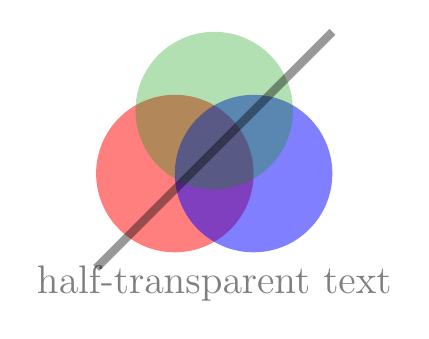
\begin{tikzpicture}
  \fill[red, opacity=0.5] (0,0) circle (1);
  \fill[blue, opacity=0.5] (1,0) circle (1);
  \fill[green!60!black, fill opacity=0.3] (0.5,0.8) circle (1);
  \draw[line width=3pt, draw opacity=0.4] (-1,-1.2) -- (2,1.8);
  \node[text opacity=0.5, font=\Large] at (0.5,-1.4) {half-transparent text};
\end{tikzpicture}

\begin{tikzpicture}
  \shade[left color=yellow, right color=purple] (0,0) rectangle (4,2);
  \shade[ball color=cyan] (5.5,1) circle (1);
\end{tikzpicture}

\section*{Rotated}
\rotatebox{90}{Rotated 90} \rotatebox{30}{Rotated 30 degrees} \rotatebox{-15}{\fbox{A box at $-15^\circ$}}
\scalebox{-1}[1]{Mirrored text} \scalebox{2}[0.7]{Squashed}

\section*{Raw PDF specials}
\special{pdf:literal q 1 0 0 RG 2 w 0 0 m 100 30 l S Q}Text after a literal line.
\special{pdf:literal q 0 0.5 0 rg 120 0 40 20 re f Q}\hspace{6cm}A green box from a literal.

\section*{Colour}
\colorbox{yellow}{Highlighted} \textcolor{blue}{blue} \textcolor[cmyk]{0,1,0,0}{CMYK magenta} \textcolor[gray]{0.5}{grey}
\fcolorbox{red}{gray!20}{framed}
\end{document}
